%%%%%%%%%%%%%%%%%%%%%%%%%%%%%%%%%%%%%%%%%%%%
% Implementación del algoritmo
%%%%%%%%%%%%%%%%%%%%%%%%%%%%%%%%%%%%%%%%%%%%

\section{Implementación}
\label{ch07:Implementar} 

Los requisitos mínimos necesarios para una implementación adecuada son los siguientes
\begin{itemize}
    \item Implementación de red neuronal y tipos de constructores.
    \item Implementación del algoritmo. 
\end{itemize}

\subsection{Implementación de redes neuronales}

El modelo  a implementar es el presentado en el algoritmo \ref{algoritmo:estructura-de-una-red-neuronal}. En virtud del \textit{composite type} de Julia \footnotetext{ Véase la \href{https://docs.julialang.org/en/v1/manual/types/}{documentación oficial}} la forma más simple y eficiente de 
declarar una red neuronal es como un nuevo tipo de dato: \textit{red neuronal} cuyos atributos sean las matrices que definen el modelo. 

En vista a la optimización en evaluación y 
entrenamiento más eficiente las matrices 
$A$ y $S$ se han escrito en una sola permitiendo así una evaluación más compacta. 
Puede encontrar la implementación 
en \href{https://github.com/BlancaCC/TFG-Estudio-de-las-redes-neuronales/tree/main/OptimizedNeuralNetwork.jl/src}{nuestro repositorio}.
\subsubsection{Diseño de test} 
Para las redes neuronales generadas de manera aleatoria se debe de satisfacer que: 
\begin{itemize}
    \item Las dimensiones de salida son las requeridas.
    \item Las matrices no deben de tener todas sus entradas idénticas, ya que ese caso tiene probabilidad nula de ocurrir. 
\end{itemize}

Para las redes neuronales generadas a partir de 
ciertas matrices: 
\begin{itemize}
    \item Que exista comprobación de tipos en la entrada.
    \item Que se cerciore de la coherencia de las matrices.
    \item  La estructura se almacena correctamente. 
\end{itemize}

\subsubsection{Ejemplo de uso}
Como ya comentamos puede encontrar un ejemplo completo de uso 
en el \href{https://github.com/BlancaCC/TFG-Estudio-de-las-redes-neuronales/blob/main/Memoria/capitulos/Ejemplo-uso-biblioteca.ipynb}{
directorio y fichero \texttt{Memoria/capitulos/Ejemplo-uso-biblioteca.ipynb}} de nuestro repositorio;
sin embargo, para mejorar la comprensión de la sección vamos a mostrar 
algunos ejemplo breves aquí.

Para construir una \textbf{red neuronal inicializada 
aleatoriamente} a partir de nuestra biblioteca
podría usarse el siguiente código: 

\begin{minipage}{\textwidth}%
    \begin{minted}
       [
        frame=single,
        framesep=10pt,
        baselinestretch=1.2,
        bgcolor=sutilBackground, 
        %linenos
       ]{Julia}
    # Dimensiones requeridas
    entry_dimension = 2
    number_of_hidden_units = 3
    output_dimension = 2
    # Creación de la red neuronal
    RandomWeightsNN(
        entry_dimension,
        number_of_hidden_units,
        output_dimension
    )
    \end{minted}
\end{minipage} 

Que tendrá como resultado la siguiente salida red neuronal de coeficientes aleatorios: 

\begin{minipage}{\textwidth}%
    \begin{minted}
       [
        frame=single,
        framesep=10pt,
        baselinestretch=1.2,
        %bgcolor=sutilBackground, 
        %linenos
       ]{Julia}
    La matrix de pesos de las neuronas, W1, es:
    3×3 Matrix{Float64}:
    0.705454   0.305242  0.46417
    0.0991484  0.720979  0.231972
    0.46869    0.683745  0.981889
    
    La matrix de pesos de la salida, W2, es:
    2×3 Matrix{Float64}:
    0.651893  0.227729  0.0385169
    0.937148  0.596889  0.0810362
    \end{minted}
\end{minipage} 

Veamos ahora la \textbf{creación de una red neuronal
a partir de matrices} 

\begin{minipage}{\textwidth}%
    \begin{minted}
       [
    frame=single,
    framesep=10pt,
       baselinestretch=1.2,
       bgcolor=sutilBackground, 
       %linenos
       ]{Julia}
    S = [1,2,3] # Matriz de sesgos
    A = [3 4 1; 4 6 3; 1 1 1] # Matriz de pesos entre entrada y capa oculta 
    B = [1 2 3; 3 2 3] # Matriz de pesos entre capa oculta y salida
    FromMatrixNN(S, A, B)
    \end{minted}
\end{minipage} 

Que tendrá como salida:

\begin{minipage}{\textwidth}%
    \begin{minted}
       [
        frame=single,
        framesep=10pt,
        baselinestretch=1.2,
        %bgcolor=sutilBackground, 
        %linenos
       ]{Julia}
    La matrix de pesos de las neuronas, W1, es:
    3×4 Matrix{Int64}:
    3  4  1  1
    4  6  3  2
    1  1  1  3

    La matrix de pesos de la salida, W2, es:
    2×3 Matrix{Int64}:
    1  2  3
    3  2  3
\end{minted}
\end{minipage}


\subsection{Implementación del algoritmo de \textit{Forward propagation}}  
La evaluación de una red neuronal se realizará por 
medio de una función que recibe como parámetros un 
tipo de dato \textit{red neuronal}.  Puede encontrar la implementación en \href{https://github.com/BlancaCC/TFG-Estudio-de-las-redes-neuronales/tree/main/OptimizedNeuralNetwork.jl/src}{nuestro repositorio}.

\subsubsection{Diseño de los tests} 
De acorde al modelo \ref{definition:redes_neuronales_una_capa_oculta} 
tomando como función de activación la identidad 
(aunque no sería una función de activación como tal)
se podrían construir fácilmente 
redes neuronales que: 
\begin{itemize}
    \item Sean la función identidad. 
    \item Actúen como una traslación.
    \item Actúen como un escalado. 
\end{itemize}
Sabiendo esto es fácil predecir para cierta entrada
cual debiera de ser su salida con el algoritmo de 
\textit{forward propagation}, esto nos va a permitir comprobar la correcta evaluación para:
\begin{itemize}
    \item Redes neuronales con matrices $A$ y $B$ diagonales. 
    \item Redes neuronales con $S$ no nulo. 
    \item Combinaciones de tipos anteriores. 
\end{itemize}
Faltaría comprobar el caso en que $A$ y $B$ no fueran diagonales, a sabiendas de que para los casos anteriores su funcionamiento es correcto, basta con comprobarlo con un ejemplo aleatorio. 

Como la evaluación es correcta falta por cerciorarse 
de que se comporta como es debido con las funciones de activación definidas. 

\subsubsection{Ejemplo de uso}
\begin{minipage}{\textwidth}%
    \begin{minted}
       [
        frame=single,
        framesep=10pt,
        baselinestretch=1.2,
        bgcolor=sutilBackground, 
        %linenos
       ]{Julia}
    # Variables auxiliares 
    # S,A,B son las matrices del ejemplo anterior 
    v = [1,2,2]
    h = FromMatrixNN(S, A, B)
    # Ejemplo de evaluación h(v) 
    # con función de activación ReLU y ForwardPropagation 
    ForwardPropagation(h, ReLU,v )
 
    \end{minted}
\end{minipage}

El resultado de las líneas anteriores sería: 

\begin{minipage}{\textwidth}%
    \begin{minted}
       [
        frame=single,
        framesep=10pt,
        baselinestretch=1.2,
        %bgcolor=sutilBackground, 
        %linenos
       ]{Julia}
    2-element Vector{Int64}:
    86
    114
    \end{minted}
\end{minipage} 

\subsection{Implementación del algoritmo de inicialización aprendida de pesos}

Se ha realizado la implementación de acorde al algoritmo descrito 
en \ref{algo:algoritmo-iniciar-pesos}. Para un desarrollo optimizado se han tenido en cuenta tres 
factores esenciales: 
\begin{itemize}
    \item Adaptación de los tipos de datos y \textit{ dispatch methods} de Julia en función 
    de las dimensiones de entrada y salida del conjunto de datos de entrenamiento.
    \item Estructuras de datos propias de Julia. 
    \item Tipo de datos de variables auxiliares. 
\end{itemize}

\subsubsection{ Uso de los tipos de datos y \textit{ dispatch methods}}
Las entradas y salidas de dimensión uno son codificadas como vectores en lugar de matrices, 
es por ello que vamos a hacer uso de la variedad de tipos que ofrece Julia y de sus \textit{dispatch methods} que ya comentamos en 
la sección \ref{ch06:sistema-timpos-julia} con
 profundidad. 

 Gracias a esta manera de implementar polimorfismo 
 en Julia, tendremos una sola función que recoja a 
 nuestro algoritmo de inicialización aprendida de pesos y diversas implementaciones adaptadas a la dimensión de entrada y salida. 

 Puede consultar la implementación en \href{https://github.com/BlancaCC/TFG-Estudio-de-las-redes-neuronales/tree/main/OptimizedNeuralNetwork.jl/src}{la carpeta \textit{weight-initializer-algorithm}} de nuestra biblioteca. 
 Cabe mencionar que el caso de entrada y salida de dimensión uno ha sido el que más reducción de costo 
 ha permitido, ya que en vez de realizar 
 el diseño directo recogido en \ref{algo:algoritmo-iniciar-pesos} puede uno consultar 
 el caso primero de la demostración  \ref{teorema:2_5_entrenamiento_redes_neuronales}
 y darse cuenta de que la existencia del vector $p$ 
 es una argucia para conseguir un orden en los vectores de entrada. Como $\R$ ya es un cuerpo ordenado, se puede prescindir tanto de $p$ como de toda la estructura de datos que ello conlleva. 
 Esta cuestión guarda relación con el apartado siguiente. 

\subsubsection{Selección de la estructuras de datos adecuada}
Como ya observamos en  la sección \ref{ch07:coste-computacional-algoritmo-propio} el coste computacional recae principalmente en conseguir una ordenación del conjunto denominado como 
$\Lambda$ en el pseudo código \ref{algo:algoritmo-iniciar-pesos}. 

La forma más eficiente de proceder en estos casos
es con una estructura de datos pertinente. 
En lenguajes como C++ una solución eficaz sería introducir los datos en 
un \textit{set}, que por estar construidos sobre un \href{https://en.wikipedia.org/wiki/Red–black_tree}{\textit{red-black tree}}
% Sobre la implementación
\footnote{ 
    Puede consultar la implementación del tipo de dato \textit{set} de la STL en 
    \url{https://github.com/gcc-mirror/gcc/blob/master/libstdc\%2B\%2B-v3/include/bits/stl_set.h}
    (fuente consultada por última vez el 8 de junio de 2022).      
}
%https://en.wikipedia.org/wiki/Red–black_tree
\marginpar{\maginLetterSize
    \iconoAclaraciones \textcolor{dark_green}{     
        \textbf{
            Estructura de datos 
            \textit{red-black tree}
        }
    }
    Se trata de un árbol binario de búsqueda 
    equilibrado, esto es un grafo no cíclico que partiendo de uno concreto denominado raíz la \textit{altura} (número máximo de nodos hasta llegar a un extremo partiendo de la raíz) es mínima. 

    Esta estructura es muy interesante ya que no solo guarda los datos ordenados si no que su coste de búsqueda es $\mathcal{O}(n \log(n))$, pero su inserción y consulta de media términos de análisis de amortización tiene complejidad constante. En el peor de los casos sería  
    $\mathcal{O}(n \log(n))$.  
}
tienen como efecto la ordenación eficiente de los mismos. 

% Sobre contribuir a Julia
\setlength{\marginparwidth}{\smallMarginSize}
\reversemarginpar
\marginpar{\maginLetterSize
    \iconoClave  \textcolor{darkRed}{     
        \textbf{
            Contribución a Julia
        }
    }
    Sería interesante explorar si se podría contribuir a Julia a partir de esta implementación, ya que a priori el uso de un diccionario solo 
    aporta simpleza en la implementación,
    \href{https://github.com/JuliaLang/julia/blob/master/CONTRIBUTING.md}{CONTRIBUTING}.
}
\setlength{\marginparwidth}{\bigMarginSize}
\normalmarginpar
Por desgracia, en Julia esto no es posible sin hacer uso de bibliotecas externas o una implementación propia; ya que el tipo conjunto está
 construido sobre diccionarios
 (ver la línea 40 de la implementación del tipo \textit{set} de Julia que puede
 encontrar en   \href{https://github.com/JuliaLang/julia/blob/master/base/set.jl}{sus fuentes en GitHub})\footnote{
     Las fuentes se encuentran concretamente en 
     \url{https://github.com/JuliaLang/julia/blob/master/base/set.jl}
     y han sido consultadas por última vez el 8 de junio de 2022.
 }.

 Para resolver el problema hemos optado 
 por usar el tipo de dato de Julia 
 \textit{Array} \footnote{
    Véase su documentación oficial 
    \url{https://docs.julialang.org/en/v1/base/arrays/}

    Consultada por última vez el 8 de junio de 2022.
}
ya que tiene los siguientes beneficios: 
\begin{itemize}
    \item Permite declarar directamente la dimensión requerida (que es conocida de antemano por tratarse del número de neuronas); esto ahorraría en evitar tener que estar redimensionando en cada inserción.
    \item Permite introducir el tipo de dato que contendrá. En la propia documentación de Julia \footnote{
        Consultar \url{https://docs.julialang.org/en/v1/manual/performance-tips/}.
        Fue visitada por última vez el 8 de Junio de 2022.
    } se nos indica que evitar el uso de tipo abstractos mejora la eficiencia. 
    \item Mantiene el mismo coste computacional.
    Concretamente para ordenar Julia dispone de
    dos algoritmos: \textit{Quick Sort} y \textit{Merge Sort}\footnote{ Consúltese \url{https://docs.julialang.org/en/v1/base/sort/}} . 

    Nosotros hemos optado por usar \textit{Quick Sort} \cite{Quicksort} porque a pesar de tener ambos algoritmos la misma complejidad media $\mathcal{O}(n \log(n))$, la constante oculta de \textit{Quick Sort} es menor con \textit{arrays}  y además no necesita de memoria adicional, (\textit{Merge Sort} \cite{merge-sort} tiene complejidad $\mathcal{O}(n)$ en memoria) (véase el artículo comparativo \cite{quicksort-vs-merge-sort}).
\end{itemize}

\subsubsection{Tipo de datos de variables auxiliares}
Se ha seleccionado cuidadosamente el tipo de las variables auxiliares.
\begin{itemize}
    \item Tipo de dato de $p$: Se ha seleccionado como un vector aleatorio de \textit{Float32}, mientras que el resto de operaciones vectoriales son de \textit{Float64}, el motivo de esto es que $p$ se operará como \textit{Float64} con una precisión mayor al no tener tantas cifras decimales. 
    \item Para otras variables auxiliares que sabemos que van a ser pequeñas se han especificado tipos como \textit{Int8}.
\end{itemize}

\subsection{Diseño de los tests} 

Deberá comprobarse que las dimensiones de salida de la red neuronal son las adecuadas 
con respecto a la entrada y salida de los datos. 

De acorde a la propiedad del teorema \ref{teo:eficacia-funciones-activation} 
todos los datos con los que se construya la red neuronal al evaluarse deben 
de tener la misma imagen.

\subsection{Ejemplo de uso}
Para crear la red neuronal bastará con llamar a la función 
\begin{verbatim}
    nn_from_data(X_train, Y_train, n, M)
\end{verbatim}
con $n$ el número de neuronas y $M$ una constante elegida según los criterios ya mencionados en \ref{table:M-activation-function} y \ref{table:M-activation-function-2}. 

Veamos un ejemplo de ejecución: 

\begin{minipage}{\textwidth}%
    \begin{minted}
       [
        frame=single,
        framesep=10pt,
        baselinestretch=1.2,
        bgcolor=sutilBackground, 
        %linenos
       ]{Julia}
       # Declaramos las variables que vamos a seguir
       # Función ideal que queremos aproximar
       f_regression(x)=(x<1) ? exp(-x)-4 : log(x)
       data_set_size = 5 
       n = data_set_size # Número de neuronas 
                         # coincide con el tamaño del conjunto
       #Partición homogénea del dominio [-3,3]
       K_range = 3
       X_train= Vector(LinRange(-K_range, K_range, n)) 
       Y_train = map(f_regression, X_train) # Imágenes de la partición
       
       M = 1
       # USO DE LA FUNCIÓN DE INICIALIZACIÓN DE LOS PESOS
       h = nn_from_data(X_train, Y_train, n, M)
       
    \end{minted}
\end{minipage} 

\begin{minipage}{\textwidth}%
    \begin{minted}
       [
        frame=single,
        framesep=10pt,
        baselinestretch=1.2,
        bgcolor=sutilBackground, 
        %linenos
       ]{Julia}
       # Imprimimos la red neuronal 
       display(Text("La red neuronal obtenida es :"))
       println(h)
       
       # Vamos a ver cómo aproxima los resultados 
       # Función que dado un punto lo evalúa con ForwardPropagation
       # y la función de activación Rampa
       evaluate(x)=ForwardPropagation(h,
               RampFunction,x)

       # Mostramos gráfica comparativa
       entre el resultado y la función ideal
       
       plot(x->evaluate([x])[1],
            -K_range,K_range, 
            label="red neuronal n=$n")
       plot!(f_regression,
           label="f ideal",
           title="Comparativa función ideal y red neuronal n=$n")
      
    \end{minted}
\end{minipage} 

El resultado ha sido el siguientes

\begin{minipage}{\textwidth}%
    \begin{minted}
       [
        frame=single,
        framesep=10pt,
        baselinestretch=1.2,
        %bgcolor=sutilBackground, 
        %linenos
       ]{Julia}
       La red neuronal obtenida es :
       La matrix de pesos de las neuronas, W1, es:
       5×2 Matrix{Float64}:
        0.0       1.0
        1.33333   3.0
        1.33333   1.0
        1.33333  -1.0
        1.33333  -3.0
       
       La matrix de pesos de la salida, W2, es:
       1×5 Matrix{Float64}:
        16.0855  -15.6038  -3.48169  3.40547  0.693147
    \end{minted}
\end{minipage} 

Además de la imagen  \ref{img:ch07-ejemplo-5-neuronas-incializacion-pesos}

\begin{figure}[H]
    \centering
     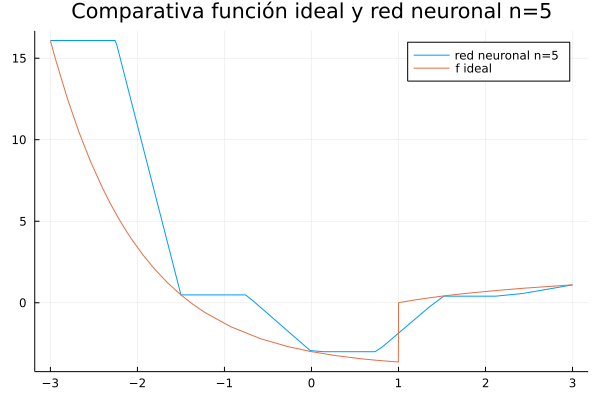
\includegraphics[width=.8\textwidth]{7-algoritmo-inicializar-pesos/f_ideal_y_rn_con_5_neuronas.png}
     \caption{Ejemplo de ejecución del algoritmo de inicialización aprendida de pesos}
     \label{img:ch07-ejemplo-5-neuronas-incializacion-pesos}
    \end{figure}



